% Chapter 2 - Social network perspective
\section{Introduction}

Firms access knowledge, resources, markets, or technologies via various social networks \citep{inkpen2005social}. The span of an organisation’s network of ties to partners (reach) and the resources that the organisation can access via its partners (richness) determine the value that it can potentially extract from its inter-organisational networks \citep{gulati2011networks}. Reach and richness bring together structural and relational properties that, together with associated organisational capabilities, explain the performance implications of networks in an integrated manner. The configuration of a firm's network ties determines how easily knowledge can be transformed into valuable innovations \citep{tortoriello2010activating}. We can use social network analysis to examine network configurations and determine the extent to which these are shaped by individual attributes and knowledge properties. This chapter describes some of the salient features of social networks and key social mechanisms for mobilising knowledge. It then introduces exponential random graph models, an advanced social network analysis technique for examining network configurations. \medskip  

\section{Social networks}

Social networks provide a way of thinking about social systems, one that focuses on the relationships among entities that make up the system \citep{borgatti2013analyzing,robins2015doing}. Networks can be represented mathematically as graphs consisting of a set of vertices and a set of edges that connect vertices \citep{newman2010networks}. \medskip

Vertices represent actors or nodes in a social network, which can be individuals, groups, organisations, regions, or even nations. Actors may be distinguished by binary, categorical or continuous attributes. For example, consider an individual actor classified as female (binary attribute), who works for a particular organisation (categorical attribute), with a specific number of years work experience (continuous attribute). \medskip

Edges represent relations or social ties between actors. Ties can be measured as directed or undirected and as binary or valued. Deciding whether to measure a tie as directed or undirected depends on the theoretical nature of the tie. For instance, co-membership is inherently undirected whereas authority is essentially directed. Directed and undirected ties can be measured as binary ties that either exist or do not exist, or as valued ties that can be stronger or weaker, transmit more or fewer resources, or have greater or lesser amount of contact \citep{scott2011sage}.\medskip

Different types of relations may exist between actors with each type of relation giving rise to a corresponding network \citep{borgatti2013analyzing}. Measuring knowledge sharing ties would, for example, generate a knowledge sharing network. Assigning an attribute to the knowledge sharing tie allows us to qualify the relationship in terms of, say, the content or frequency of knowledge sharing (e.g. how much of the knowledge be shared is tacit in nature). \medskip

Figure \ref{fig:tie_type} characterises different types of social ties. Ties between actors who share something in common (e.g. work at the same location, are affiliated to the same body, participate in the same event, or share a common attribute) are referred to as similarity ties. Relational ties include kinship and other ties, such as friendship, advice, and managerial ties. Relational cognition refers to ties that are affective (e.g. like or dislike another actor) or perceptual (e.g. belief about the other actor) in nature. Relational events refer to ties defined by specific social interactions (e.g. a transaction of some kind) and flows (e.g. knowledge flows). \medskip

\begin{figure}
	\centering
	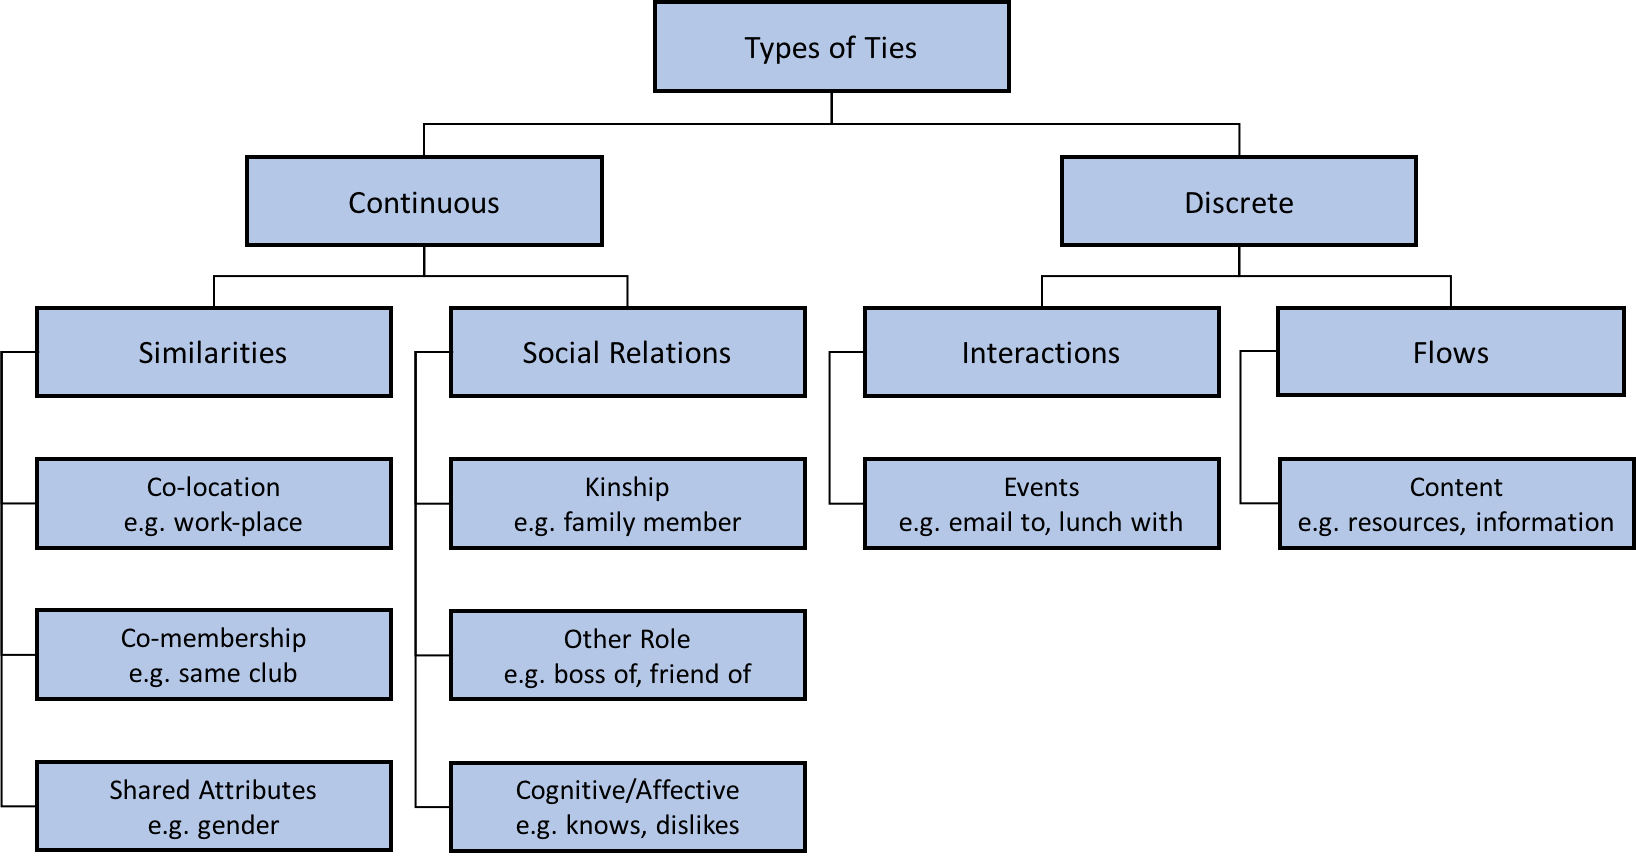
\includegraphics[width=0.9\linewidth]{tie_type}
	\caption{Different types of ties. Modified after \citet{borgatti2009network}.}
	\label{fig:tie_type}
\end{figure}

Actors who know each other well are said to have strong ties with one another. Ties that are characterised by infrequent interaction, short histories, and limited emotional closeness may be characterised as weak ties \citep{baer2010strength}. Some ties are dependent on others. An example is friendship, which usually develops because of an pre-existing similarity tie (e.g. both actors live in the same neighbourhood, attend the same school, or work at the same place) or via a relational event tie (e.g. actors were introduced to each other at a specific event or worked together on a particular project). Actors are more likely to share knowledge (relational event) with others who have common interests (similarity tie) or with others they trust (relational cognition). Multiplex relations between two actors are considered to be stronger because their redundancy can make them endure the rupture of a specific type of connection \citep{dickison2016multilayer}. \medskip 

\section{Social network analysis}

The aim of social network analysis is detecting and interpreting patterns of social ties between actors \citep{wasserman1994social,de2011exploratory}. Most basic questions in social network analysis involve the measurement and modelling of particular structural properties such as reciprocity, degree distribution, triadic closure, and homophily \citep{butts2008social,snijders2011statistical}. To fully understand the implications of dyadic relations between actors, one has to consider how these are shaped by broader patterns of social interaction \citep{scott2011sage}. This requires more than simply measuring the basic characteristics of networks. A set of assumptions is needed to best describe and explain social phenomena of interest. This may involve applying an existing psychological or social theory to develop propositions or test hypotheses about specific social relations \citep{scott2011sage,borgatti2013analyzing}. \medskip

Actors in knowledge networks serve both as keepers of knowledge and as agents that seek out, communicate, and create knowledge \citep{phelps2012knowledge,pugh2013designing}. Knowledge by itself is simply a latent resource. It only becomes valuable once it is mobilised and used \citep{marabelli2012knowledge,freeman2015knowledge}. Examining the local configuration of knowledge networks can shed light on the social processes that transform new knowledge into innovations. \medskip

For instance, actors that know each other well are said to have strong ties with one another. Such actors tend to have similar interests and are privy to the same knowledge. Strong ties tend to make people look inward and not be very receptive to external knowledge. Casual acquaintances, on the other hand, can be regarded as weak ties. Because acquaintances usually mix in different social circles, weak ties are more likely to provide actors access to new knowledge and opportunities \citep{granovetter1973strength}. \medskip

Knowledge networks with an abundance of weak ties are typically sparse with many disconnected parts or \enquote{structural holes} \citep{burt1992structural}. Actors who bridge otherwise disconnected parts of the knowledge network are termed knowledge brokers. Brokerage may be defined as the \enquote{behaviour by which an actor influences, manages, or facilitates interactions between other actors} \citep{obstfeld2014brokerage}. Knowledge brokers make connections between those who need knowledge and those who have it \citep{davenport1998successful}. They are able to identify and establish strategic relationships with keepers of knowledge. Some knowledge brokers exploit this to their own advantage while others try establish new relations between otherwise disconnected people \citep{gould1989structures,burt1992structural,obstfeld2014brokerage}. One can assess how actors exercise power by examining patterns of brokerage in knowledge sharing networks. \medskip

Reciprocity is a key concept in social exchange and game theory that reflects a human tendency to return helpful or harmful acts in kind \citep{nowak2005evolution}. Both social exchange and game theory suggest dyadic relationships have a tendency to be symmetrical \citep{emerson1976social,axelrod1984evolution}. In other words, reciprocity leads to balanced and more stable relations, which in turn helps build trust and strengthen ties between actors \citep{blau1964exchange}. Non-reciprocated or asymmetric ties are more likely to be unstable i.e. are unlikely to be long-lasting or strong \citep{snijders2011statistical}. \medskip %Past studies show that people are more inclined to share knowledge with others if this behaviour is reciprocated \citep{ipe2003knowledge}. \medskip

Past studies show that when new actors join a social network, there is an attachment bias i.e. actors are more likely to connect with other actors who are already quite popular. This is also referred to as \enquote{preferential attachment} \citep{barabasi1999emergence}. The implication of such a bias is that well-connected actors will increase their connectivity at a higher rate than less well-connected actors, the so-called \enquote{rich-get-richer} phenomenon \citep{desollaprice976general}. In other words, preferential attachment suggests that some people in a knowledge exchange network will acquire knowledge at a faster rate than others. Given that knowledge is a source of power, this has implications for power-dependence relations. More central actors are able to exert much more influence because they have greater access to diverse knowledge \citep{emerson1962power,bonacich1987power}. \medksip 

Sociologists are particularly interested in group processes and how these impact individual perceptions and behaviour \citep{de2011exploratory}. Balance theory argues people feel uncomfortable when they think their friends do not like each other \citep{heider1958psychology}. To resolve this discomfort, the theory predicts that one will either discard a friend, or more likely, one will change one’s perceptions of the relationship between friends to restore cognitive balance i.e. \enquote{a friend of a friend is a friend of mine} \citep{krackhardt1987cognitive}. Achieving structural balance in social relations typically results in triadic or transitive closure, which can be either cyclic or hierarchical in nature. Cyclic closure tends to relatively low in social networks, indicating the pervasiveness of hierarchies in local group structures \citep{davis1967structure}. \medskip  

Homophily is the tendency of similar actors to relate to each other \citep{mcpherson2001birds}. Theoretical arguments can be based on opportunity, affinity, ease of communication, reduced transaction costs and break-off risks, and organisational foci composed of similar individuals. This leads to a higher probability of ties being formed between actors with similar values on relevant covariates \citep{snijders2011statistical}. \medskip

\section{Exponential random graph models}

Exponential random graph models (ERGMs) are a class of statistical model for social networks originally developed by \citet{frank1986markov} and refined by \citet{wasserman1996logit} and \citet{pattison1999logit}. ERGMs have the capacity to address complex social structures. Recent model derivations are able to examine both individual-level variables and structural relations simultaneously \citep{robins2007recent}. \medskip

An ERGM is essentially a pattern recognition device which breaks a network down into its constituent network motifs or configurations and then test if particular configurations occur more or less frequently than would be expected by chance alone. Network configurations are patterns of social network ties assumed to represent underlying social processes or mechanisms \citep{lusher2014cooperative}. For example, a theory may suggest that actors with specific attributes are more likely to receive social ties. This can be tested using an ERGM to see if actors with such attributes are receiving more ties than would be expected by chance alone. That way, a researcher can test certain hypotheses or propositions about tie formation relating to theory \citep{robins2007recent}. \medskip

ERGMs permit differentiation between structural network effects and processes related to actor attributes. Unlike the assumption of independence of observations in standard statistical tests, ERGMs are based on the assumption of conditional dependence \citep{pattison2002neighborhood}. An ERGM is similar to a logistic regression, but is more sophisticated because it can handle complex dependency assumptions. This reflects social reality where ties are largely interdependent \citep{kadushin2012understanding}. \medskip

Purely structural effects reflect self-organising or endogenous processes in which ties form due to the presence or absence of other ties. In the case of reciprocity, for example, because one person has first done someone a favour, that other person is more likely to reciprocate the favour (\enquote{you scratch my back because I have scratched yours}). One tie follows on from the other i.e. one tie is dependent upon the other. Ties may also form due to actor attributes and are known as actor-relation effects in ERGMs. The tendency of individuals to associate and bond with similar others (also known as \enquote{homophily}) is an example of an actor-relation effect. \medskip 

\begin{table}[]
	\tiny
	\centering
	\caption{Exponential random graph model parameters used in this study.}
	\label{erm_params}
	\begin{tabular}{lcl}
		\toprule
		Parameter & Graphic & Explanation  \\ \midrule
		\textbf{Purely structural effects} & & \\
		Arc (edge)                    	& \begin{minipage}{.2\textwidth} \centering 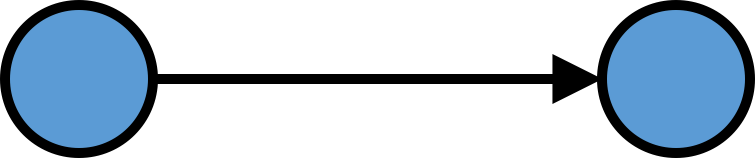
\includegraphics[width=0.4\linewidth]{Images/Arc} \end{minipage} 					& \begin{tabular}[c]{l}Baseline propensity for a tie to form in the absence of other\\ effects.\end{tabular} \\ \\
		Reciprocity (mutuality)       	& \begin{minipage}{.2\textwidth} \centering 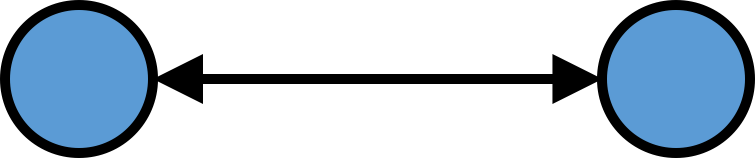
\includegraphics[width=0.4\linewidth]{Images/Reciprocity} \end{minipage} 			& \begin{tabular}[c]{l}Propensity for a tie from one actor to a second when there\\ is already a tie from the second to the first.\end{tabular} \\ \\                                                                                                       \\
		TwoPath (simple connectivity) 	& \begin{minipage}{.2\textwidth} \centering \includegraphics[width=0.4\linewidth]{Images/Twopath} \end{minipage}        		& \begin{tabular}[c]{l}Propensity for ties to form as part of simple path formations. \end{tabular} \\ \\
		AinS (popularity spread)      	& \begin{minipage}{.2\textwidth} \centering 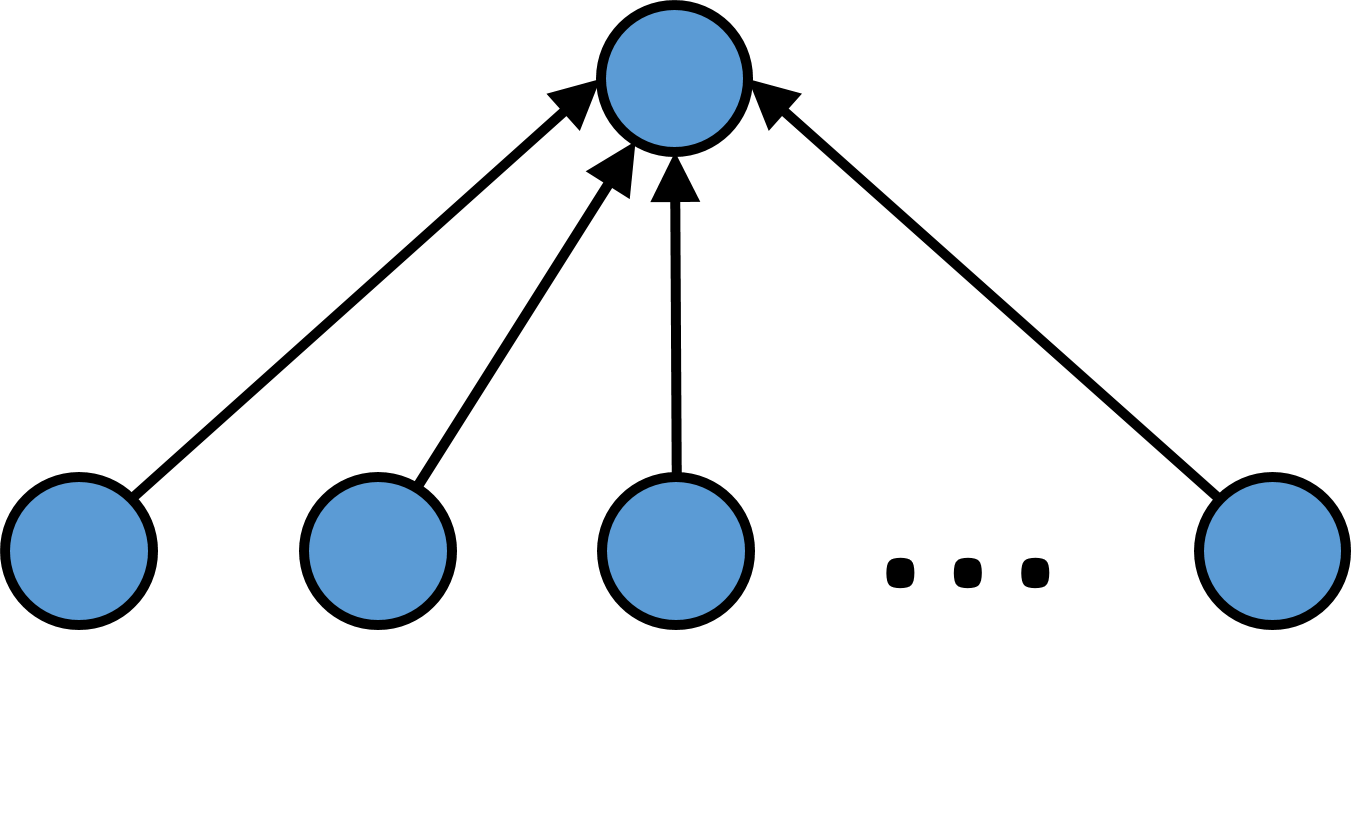
\includegraphics[width=0.6\linewidth]{Images/AinS} \end{minipage}        			& \begin{tabular}[c]{l}Propensity for dispersion in the in-degree distribution,\\ indicating there are a few highly popular actors. \end{tabular} \\ \\
		AoutS (activity spread)       	& \begin{minipage}{.2\textwidth} \centering 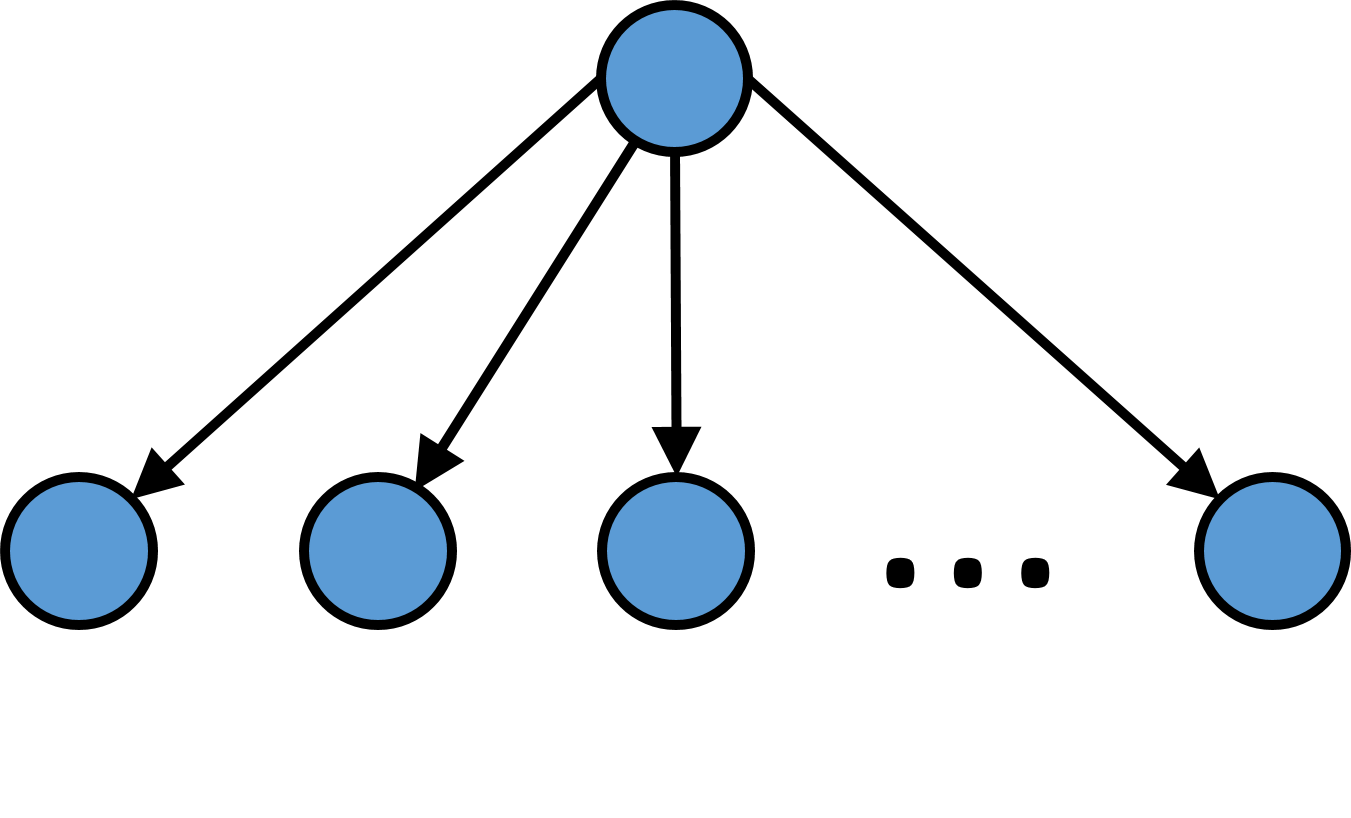
\includegraphics[width=0.6\linewidth]{Images/AoutS} \end{minipage}  				& \begin{tabular}[c]{l}Propensity for dispersion in the out-degree distribution,\\ indicating there are a few highly active actors. \end{tabular}  \\ \\
		AT-T (path closure)           	& \begin{minipage}{.2\textwidth} \centering 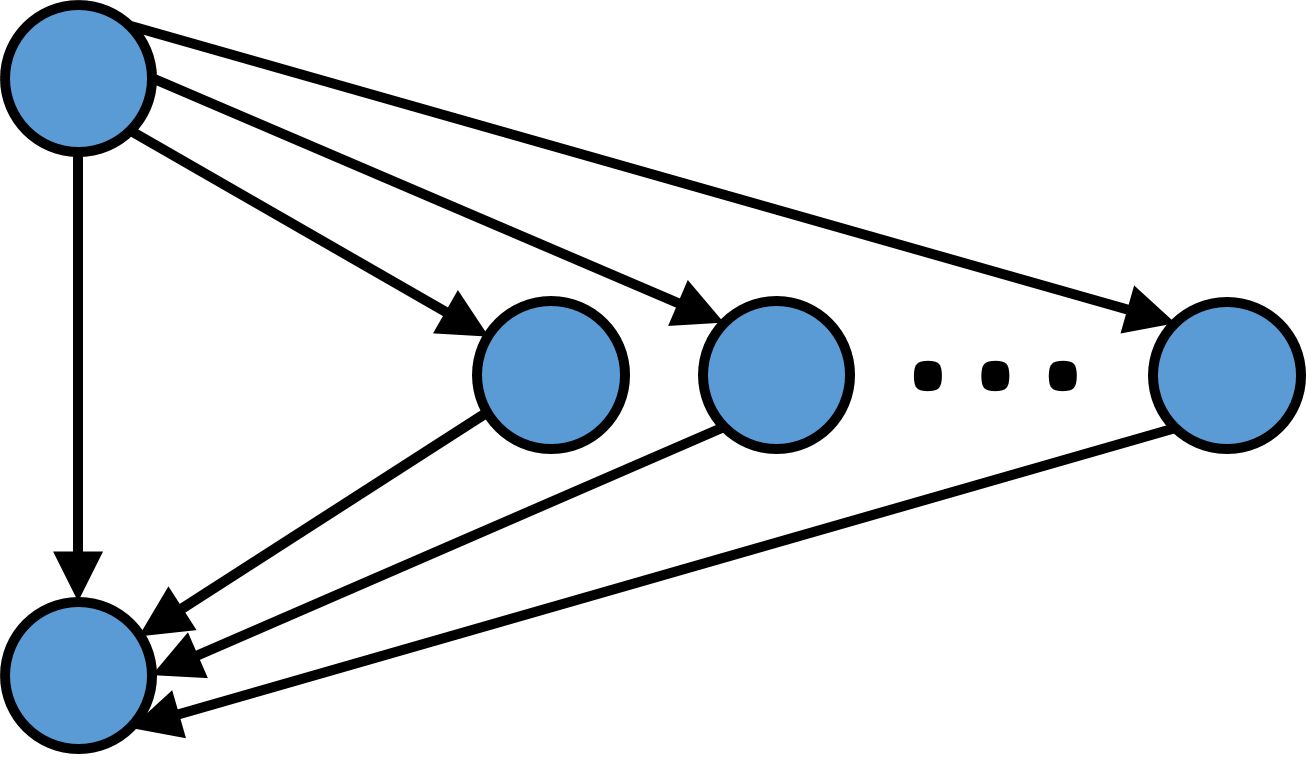
\includegraphics[width=0.6\linewidth]{Images/AT-T} \end{minipage}        			& \begin{tabular}[c]{l}Propensity for ties to form as part of transitive triad or a\\ multiple transitive configuration. \end{tabular} \\ \\
		AT-C (cyclic closure)         	& \begin{minipage}{.2\textwidth} \centering 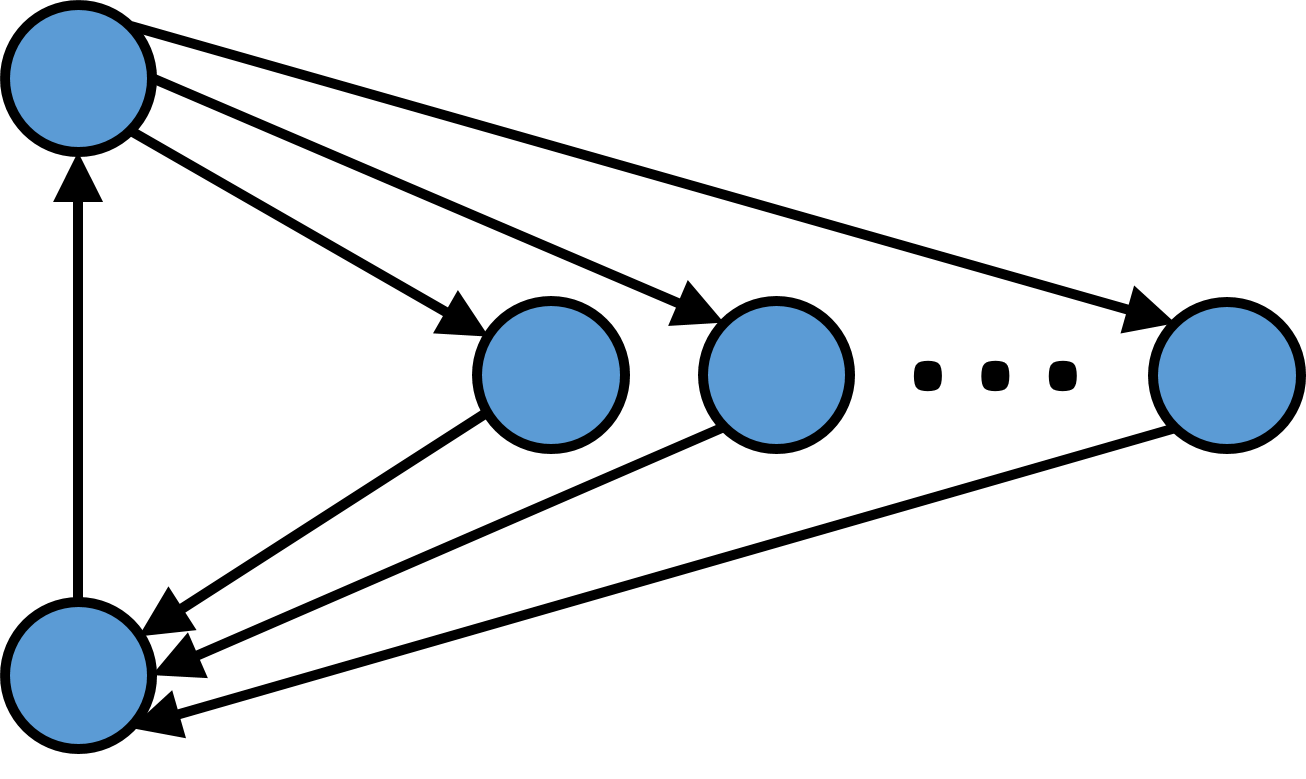
\includegraphics[width=0.6\linewidth]{Images/AT-C} \end{minipage}        			& \begin{tabular}[c]{l}Propensity for ties to form as part of a cyclic triad or a\\ multiple cyclic configuration. \end{tabular} \\ \\
		A2P (multiple connectivity)   	& \begin{minipage}{.2\textwidth} \centering 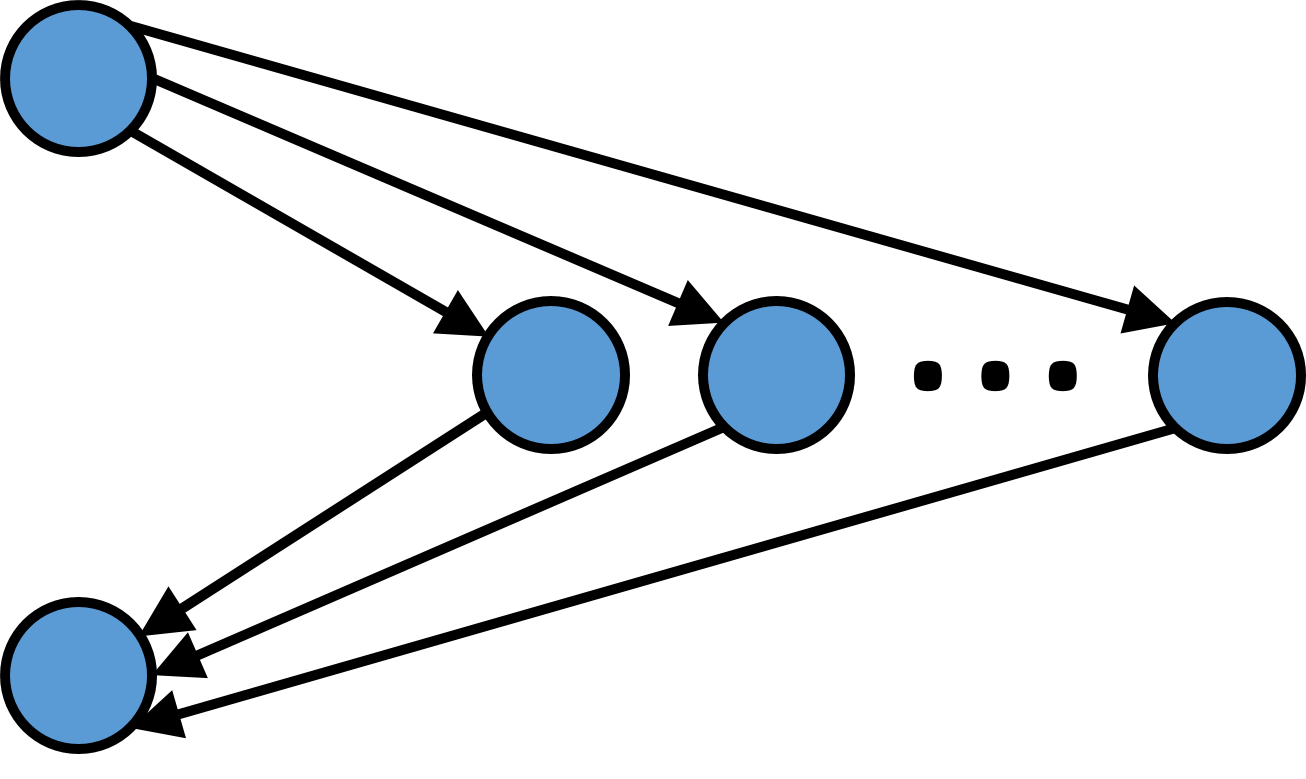
\includegraphics[width=0.6\linewidth]{Images/A2P} \end{minipage}       				& \begin{tabular}[c]{l}Propensity for ties to form as part of formations involving\\ multiple short paths between actors. \end{tabular} \\ \\
		\textbf{Actor-relation effects} & & \\
		Attribute sender              	& \begin{minipage}{.2\textwidth} \centering 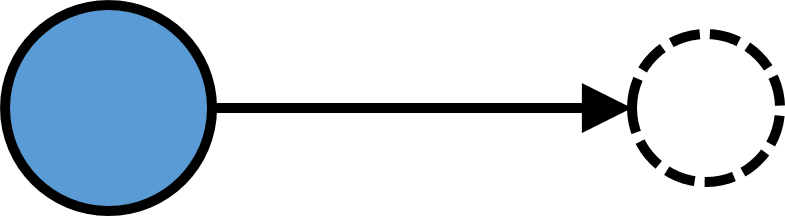
\includegraphics[width=0.4\linewidth]{Images/Sender} \end{minipage}        			& \begin{tabular}[c]{l}Propensity for a tie to be directed from an actor with a\\ particular attribute. \end{tabular} \\ \\
		Attribute receiver             	& \begin{minipage}{.2\textwidth} \centering 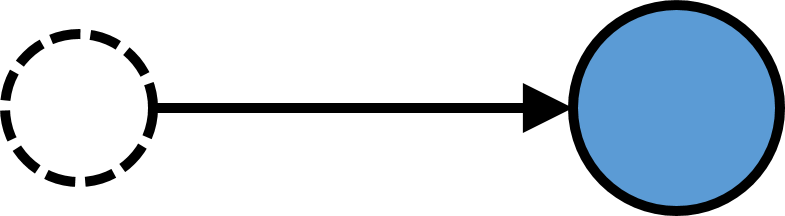
\includegraphics[width=0.4\linewidth]{Images/Receiver} \end{minipage}        		& \begin{tabular}[c]{l}Propensity for a tie to be directed toward an actor with a\\ particular attribute. \end{tabular} \\ \\
		Attribute match               	& \begin{minipage}{.2\textwidth} \centering 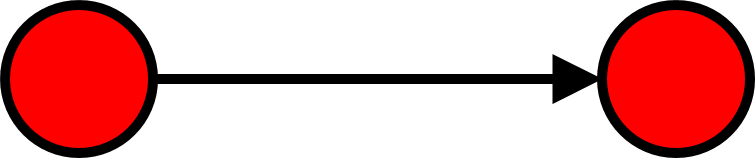
\includegraphics[width=0.4\linewidth]{Images/Match} \end{minipage}       			& \begin{tabular}[c]{l}Propensity for a tie to form between actors with the same\\ categorical attribute.\end{tabular} \\ \\
		Attribute mismatch reciprocity 	& \begin{minipage}{.2\textwidth} \centering 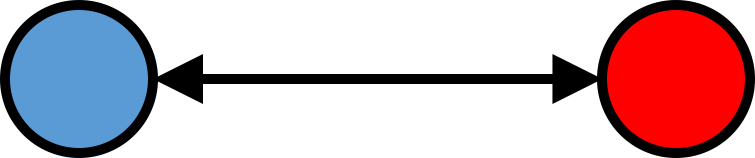
\includegraphics[width=0.4\linewidth]{Images/MisMatchReciprocity} \end{minipage}  	& \begin{tabular}[c]{l}Propensity for a tie to form between actors with a\\ non-matching categorical attribute.\end{tabular} \\ \\
		Attribute difference          	& \begin{minipage}{.2\textwidth} \centering 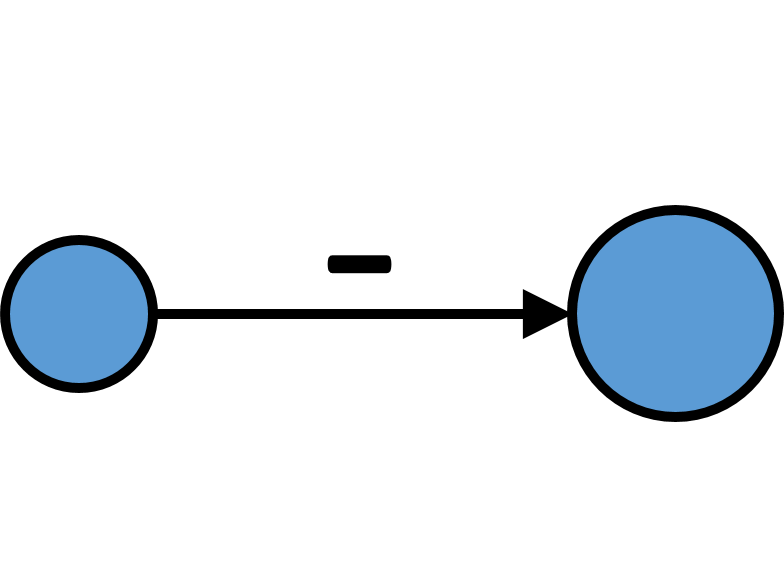
\includegraphics[width=0.4\linewidth]{Images/Difference} \end{minipage}       		& \begin{tabular}[c]{l}Propensity for a tie to form between actors with a similar\\ continuous attribute. \end{tabular} \\ \\
		Attribute product             	& \begin{minipage}{.2\textwidth} \centering 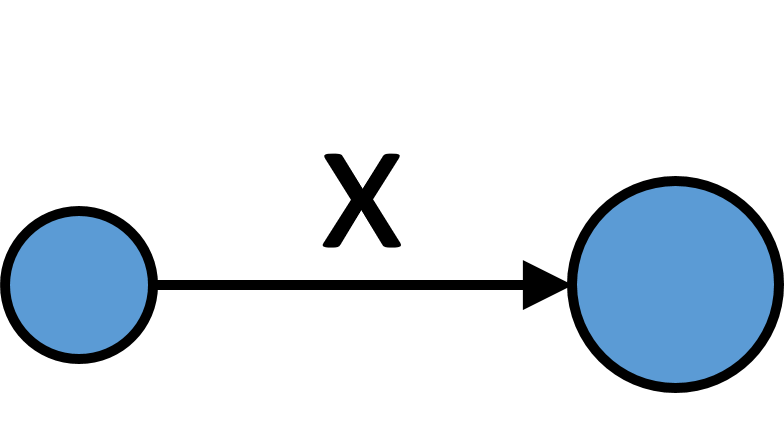
\includegraphics[width=0.4\linewidth]{Images/Product} \end{minipage}        		& \begin{tabular}[c]{l}Propensity for a tie to form between actors who both score\\ highly on the same continuous attribute. \end{tabular} \\ \\
		\textbf{Actor-brokerage effects} & & \\
		b\textsubscript{O} (liaison role)			      	&  \begin{minipage}{.2\textwidth} \centering 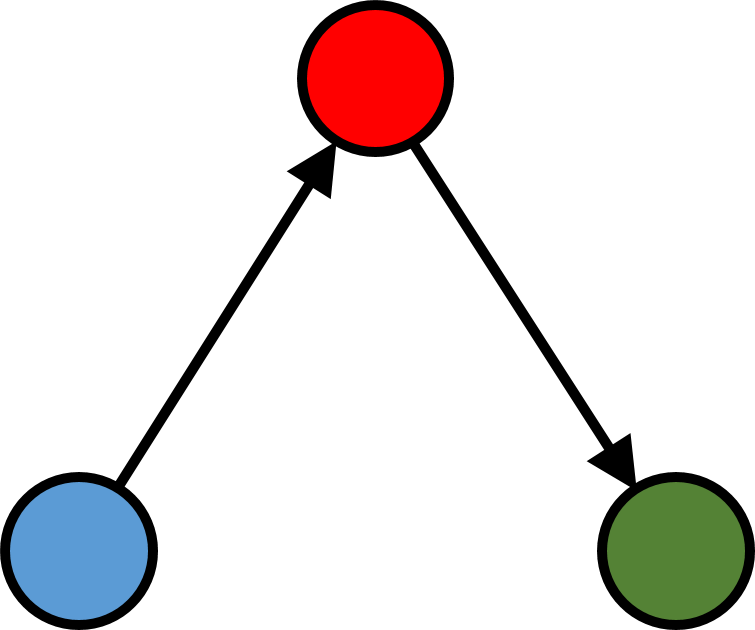
\includegraphics[width=0.4\linewidth]{Images/b_O} \end{minipage}   & \begin{tabular}[c]{l}Propensity to have brokers who mediate communication\\ between two individuals from different groups, neither of\\ which they belong to.\end{tabular}\\ \\
		b\textsubscript{IO} (representative role)		   	& \begin{minipage}{.2\textwidth} \centering 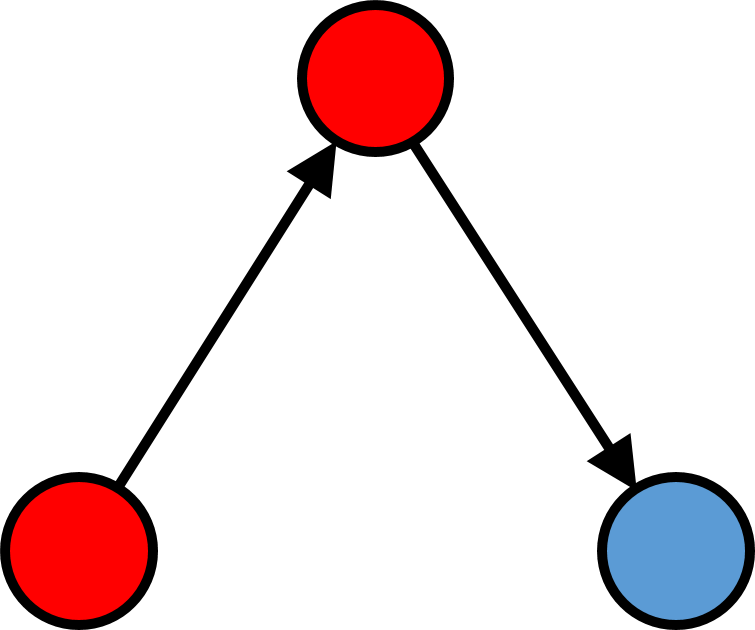
\includegraphics[width=0.4\linewidth]{Images/b_IO} \end{minipage}   & \begin{tabular}[c]{l}Propensity to have brokers who mediate communication\\ from in-group members to out-group members.\end{tabular}\\ \\
		b\textsubscript{OI} (gatekeeper role) 				& \begin{minipage}{.2\textwidth} \centering 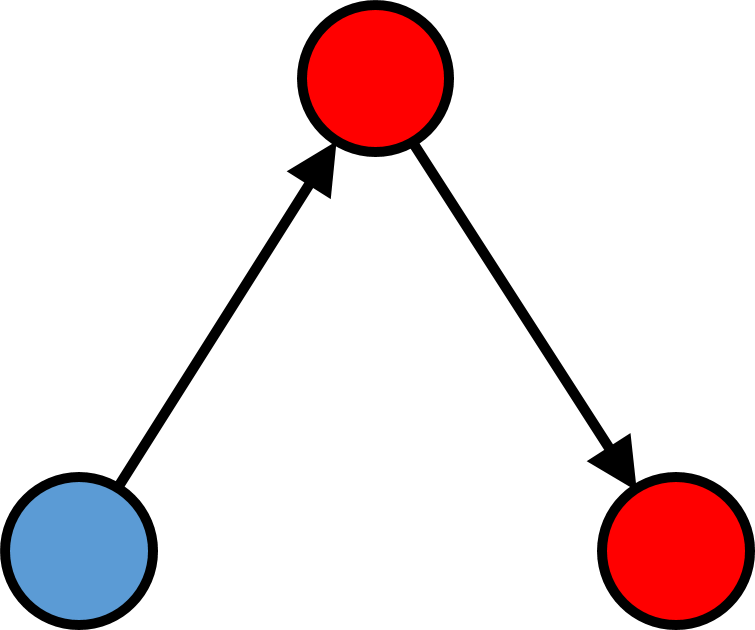
\includegraphics[width=0.4\linewidth]{Images/b_OI} \end{minipage}   & \begin{tabular}[c]{l}Propensity to have brokers who mediate communication\\ from out-group members to in-group members. \end{tabular}\\ \\
		w{\textsubscript{O}} (itinerant broker)			&  \begin{minipage}{.2\textwidth} \centering 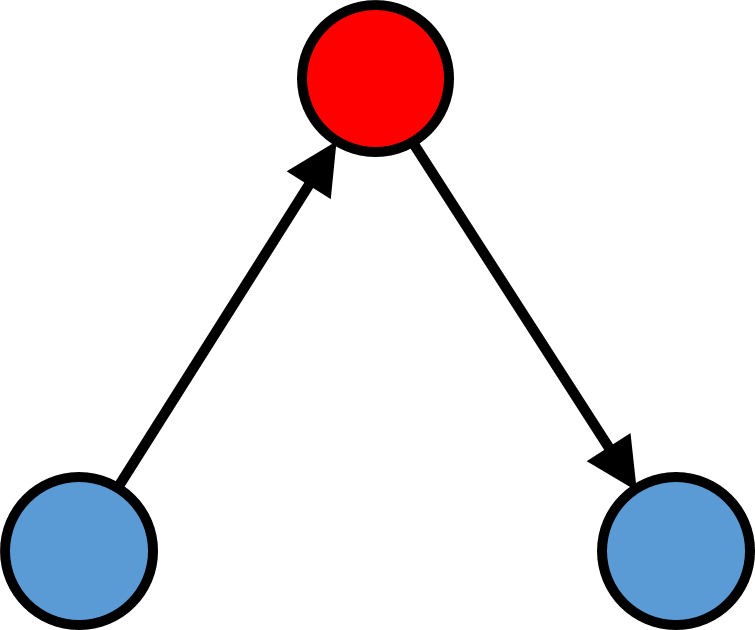
\includegraphics[width=0.4\linewidth]{Images/w_O} \end{minipage}   & \begin{tabular}[c]{l}Propensity to have brokers who mediate communication\\ between two individuals from a single group to which they\\ do not belong. \end{tabular}\\ 
		w\textsubscript{I} (coordination role)				& \begin{minipage}{.2\textwidth} \centering 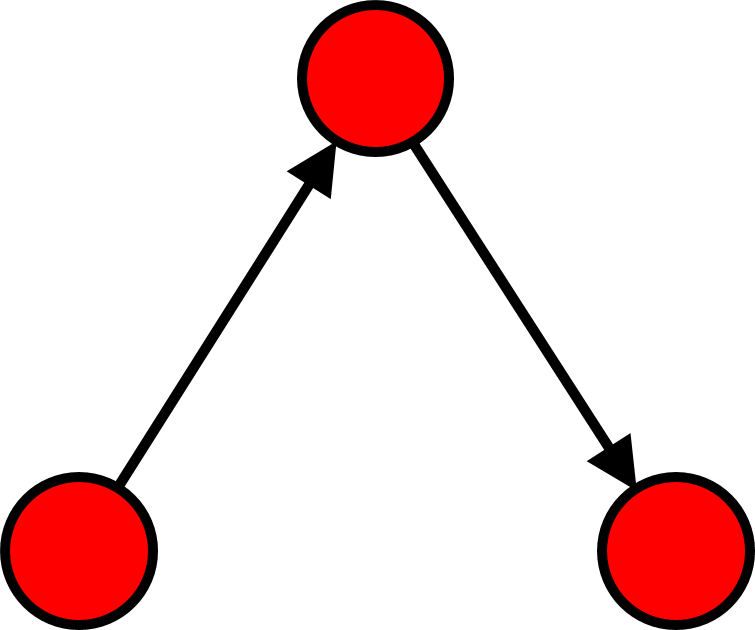
\includegraphics[width=0.4\linewidth]{Images/w_I} \end{minipage}    & \begin{tabular}[c]{l}Propensity to have brokers who mediate communication\\ between two individuals from his or her own group. \end{tabular}\\ \\	
		\textbf{Network covariate effects} & & \\
		Dyadic covariate             	& \begin{minipage}{.2\textwidth} \centering 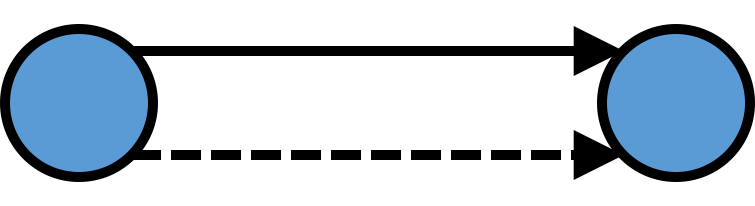
\includegraphics[width=0.4\linewidth]{Images/DyadicCovariate} \end{minipage}    	& \begin{tabular}[c]{l}Propensity for a tie of one type to form from one actor to\\ another if a tie of another type is already present, though\\ the covariate network is fixed (i.e. exogenous) in the\\ model, and so cannot vary. \end{tabular} \\\bottomrule                                                                                                       
	\end{tabular}
\end{table}

ERGMs provide a more principled way of making inferences about the association between actor attributes and network ties because ERGMs can distinguish between ties formed due to actor attributes or whether an actor’s popularity is the result of being embedded within other purely structural network structures \citep{lusher2013exponential}. Alternative methods used to assess the effect of actor attributes on network structures, such as linear regression, are unable to make such distinctions, and are thus more limited regarding the conclusions such methods can draw. ERGMs also allow multiple explanations for network tie formation to be examined simultaneously in one model, comparing one effect against another to see which is more likely to be associated with the formation of network ties (e.g. is it age or experience that matters in advice-seeking?). \medskip

\section{Conclusion}

The micro-structure of knowledge-sharing networks should reveal much regarding the social mechanisms of knowledge acquisition, assimilation, transformation, and application \citep{reagans2003network,phelps2012knowledge,tortoriello2010activating,tortoriello2015social}. For example, a researcher could examine how individual attributes and knowledge properties relate to specific patterns of social interaction. The influence of power-relations on absorptive capacity can be assessed by examining patterns of knowledge brokerage \citep{burt2004structural,obstfeld2005social,obstfeld2014brokerage}. Examining closure in tacit knowledge networks can help explain knowledge assimilation processes and the level of collaboration. Chapter 3  introduces social network analysis and explains how this can be used to assess practices that build absorptive capacity in open-innovation collaborations. 

Clarifying the implications of closed versus disconnected network structures for various organisational outcomes is important to our understanding of network resources \citep{ahuja2000collaboration}. \medskip

%Table